\documentclass[tikz]{standalone}
\usepackage{tikz}
\usepackage{tikz-qtree,tikz-qtree-compat}
\usetikzlibrary{matrix}

\begin{document}
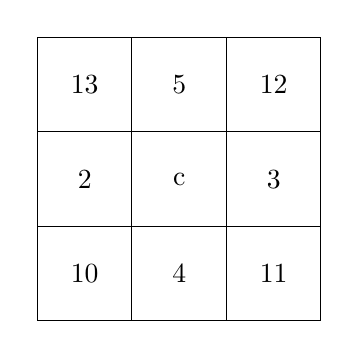
\begin{tikzpicture}
 \tikzset{square matrix/.style={
    matrix of nodes,
    column sep=-\pgflinewidth, row sep=-\pgflinewidth,
    nodes={draw,
      minimum height=#1,
      anchor=center,
      text width=#1,
      align=center,
      inner sep=0pt
    },
  },
  square matrix/.default=1.2cm
}
\matrix[square matrix]
{
   13 & 5 & 12\\
   2 & c & 3 \\
   10 & 4 & 11 \\
};
\end{tikzpicture}
\end{document}
